% Kopfzeile beim Kapitelanfang:
\fancypagestyle{plain}{
%Kopfzeile links bzw. innen
\fancyhead[L]{\Large Vorlesung 5 (28.10.2013)}
%Kopfzeile rechts bzw. außen
\fancyhead[R]{}}
%Kopfzeile links bzw. innen
\fancyhead[L]{\Large Vorlesung 5 (28.10.2013)}
%Kopfzeile rechts bzw. außen
\fancyhead[R]{}
% **************************************************
\section{Definition: Supremum, Infimum}\label{3.10}
Sei $M \subseteq \R$.
\en{
\item $s \in \R$ heißt \underline{Supremum von $M$} $\Leftrightarrow s$ ist kleinste obere Schranke von $M$.\\
Das heißt:
\begin{enumerate}[label=\roman*.]
\item $s$ ist obere Schranke von $M$.
\item $s \le s'$ für jede weitere obere Schranke $s'$ von $M$.
\end{enumerate}
\item $t \in \R$ heißt \underline{Infimum von $M$} $\Leftrightarrow t$ ist größte untere Schranke von $M$.
}
1.ii. zeigt: $M$ hat höchstens ein Supremum $s$ (bezeichnet mit $s = \text{sup } M$),\\
denn: $s, s'$ seien Suprema $\Rightarrow s \le s' \wedge s' \le s \Rightarrow s=s'$\\
Analog: $M$ hat höchstens ein Infimum $t$ (bezeichnet mit $t = \text{inf } M$).

\subsection*{Beispiel}
$M = [0,1] \Rightarrow 1 = \text{sup } M$ (denn: $1$ ist obere Schranke, und kein $x<1$ ist obere Schranke).

\section{\texorpdfstring{Vollständigkeitsaxiom: Supremumseigenschaft von $\R$}{Vollständigkeitsaxiom: Supremumseigenschaft von \R}}\label{3.11}
Sei $M \subseteq \R, M \neq \emptyset$ nach oben beschränkt $\Rightarrow M$ besitzt ein Supremum.

\section{\texorpdfstring{Folgerung aus der Supremumseigenschaft von $\R$}{Folgerung aus der Supremumseigenschaft von \R}}\label{3.12}
Sei $M \subseteq \R, M \neq \emptyset$ nach unten beschränkt $\Rightarrow M$ beistzt ein Infimum.\\
Betrachte $-M = \{-x : x \in M\}$. $-M$ hat ein Supremum $s$, da es nach oben beschränkt ist.\\
Also hat $M$ ein Infimum $-s$.\nl
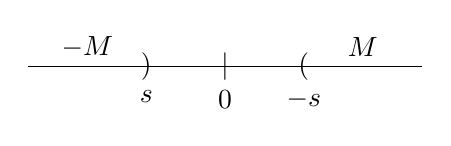
\begin{tikzpicture}[decoration=brace]
\draw(0,0)--(5,0);
\foreach \x/\xtext in {1.5/$s$,2.5/$0$,3.5/$-s$}
  \draw(\x,-5pt) node[below] {\xtext};
\draw(2.5,0pt) node{$|$};
\draw(1.5,0pt) node{)};
\draw(3.5,0pt) node{(};
\draw(0.75,7pt) node{$-M$};
\draw(4.25,7pt) node{$M$};
\end{tikzpicture}

\subsection*{Beispiel}
$M=(-3,2] \Rightarrow \text{inf } M = -3$

\subsection*{Beachte}
Hat $M$ ein Maximum $m=\text{max } M$, so ist zugleich $m=\text{sup } M$,\\
denn: $x<m \Rightarrow x \text{ ist keine obere Schranke für } M$.

\section{Lemma}\label{3.13}
Sei $M \subseteq \R, M \neq \es$ nach oben beschränkt und $s = \text{sup }M$.\\
$\Rightarrow \forall \eps>0 \exists x \in M:s-\eps<x \le s$

\subsection*{Beweis}
$s-\eps$ ist keine obere Schranke von $M$ (da $s$ schon die kleinste obere Schranke ist).\\
$\Rightarrow \exists x \in M:s-\eps<x$ Dabei ist $x \le s$, da obere Schranke von $M$. \qed

\section{\texorpdfstring{Satz: Archimedische Eigenschaft von $\R$}{Satz: Archimedische Eigenschaft von \R}}\label{3.14}
\begin{enumerate}[label=(AR)]
\item $\forall x \in \R \exists n \in \N : n > x$\\
\begin{tikzpicture}[decoration=brace]
\draw[->](0,0)--(5,0);
\foreach \x/\xtext in {1.5/$0$,3.5/$x$,4.5/$n$}
  \draw(\x,-5pt) node[below] {\xtext};
\draw(1.5,0pt) node{$|$};
\draw(3.5,0pt) node{$|$};
\draw(4.5,0pt) node{$|$};
\end{tikzpicture}
\end{enumerate}

\subsection*{Beweis durch Widerspruch}
Angenommen, (AR)  gelte nicht, also:\\
$\exists x \in \R : n \le x \forall n \in \N$\\
$\Rightarrow \N$ ist (durch $x$) nach oben beschränkt $\Rightarrow s = \text{sup } \N$ existiert.\\
$\Rightarrow$ (nach Lemma 3.13) $\exists n \in \N : s-1 < n$ ($\eps = 1$)\\
$\Rightarrow \underbrace{n+1}_{\in \N} > s$ \wspruch \qed

\section{\texorpdfstring{Folgerungen aus der archimedischen Eigenschaft von $\R$}{Folgerungen aus der archimedischen Eigenschaft von \R}}\label{3.15}
\en{
\item $\forall \eps > 0 \exists n \in \N : \frac{1}{n} < \eps$
\item Wachstum von Potenzen:\\
Sei $a \in \R, a > 1 \Rightarrow \forall M > 0 \exists n \in \N : a^n > M$
\item Sei $a \in \R, 0 < a < 1 \Rightarrow \forall \eps > 0 \exists n \in \N : a^n < \eps$\\
\begin{tikzpicture}[decoration=brace]
\draw[->](0,0)--(5,0);
\foreach \x/\xtext in {0.0/$0$,0.5/$a^n$,1.0/$\eps$,3.5/$a$,4.5/$1$}
  \draw(\x,-5pt) node[below] {\xtext} (\x,0pt) node{$|$};
\end{tikzpicture}
}

\subsection*{Beweis}
\en{
\item Sei $\eps > 0$. Dann: (AR) $\Rightarrow \exists n \in \N : n > \frac{1}{\eps} \Rightarrow \frac{1}{n} < \eps$
\item Sei $M>0$. $x = a-1 > 0 \Rightarrow a^n=(1+x)^n > 1+nx > nx \forall n \in \N$\\
(AR) $\Rightarrow \exists n \in \N : n > \frac{M}{x} \Rightarrow a^n > M$
\item Sei $\eps>0$. $\frac{1}{a}>1 \underset{\text{(2)}}{\Rightarrow} \exists n \in \N : \left(\frac{1}{a}\right)^n > \frac{1}{\eps} \Rightarrow a^n < \eps$
} \qed \nl
Man kann sagen: Es gibt (bis auf Umbenennungen) genau einen angeordneten Körper,\\
der das Vollständigkeitsaxiom erfüllt, nämlich $\R$.

\newpage

\section*{\texorpdfstring{Wichtige Konsequenz der Vollständigkeit von $\R$:}{Wichtige Konsequenz der Vollständigkeit von \R:}}
\section{Satz: Existenz von Wurzeln}\label{3.16}
Sei $a \in \R, a \ge 0$ mit $k \in \N \Rightarrow \exists! x \in \R , x \ge 0 : x^k = a$

\subsection*{Schreibweise}
$x=a^{\frac{1}{k}} = \sqrt[k]{a}$ (sprich: $k$-te Wurzel aus $a$)\\
$\sqrt[2]{a} = \sqrt{a}$

\subsection*{Beachte}
$\sqrt[k]{0}=0$ und $\forall a>0$ ist $\sqrt[k]{a}>0$ (per Definition)

\subsection*{Beweis}
\en{
\item \underline{Eindeutigkeit}:\\
Seien $x_1 , x_2 \ge 0, x_1 \neq x_2$ mit $x_1^k = a = x_2^k$.
Sei etwa $x_1 < x_2 \underset{\text{3.4}}{\Rightarrow} x_1^k < x_2^k$ \wspruch
\item \underline{Existenz}:\\
Hier für $k=2$ ($k>2$ ähnlich, etwas aufwendiger).\\
Sei ohne Einschränkung \emph{(kurz: o.e.)} $a \ge 1$.\\
(Für $a=0$ klar; für $0<a<1$ betrachten wir den Kehrwert $\frac{1}{a}>1$.\\
Ist $y^k = \frac{1}{a} \underset{y \neq 0}{\Rightarrow} (\frac{1}{y})^k = a$)\\
Setze $M := \{y>0 : y^2 \le a\}$. $M \neq \es$ (da $1 \in M$) ist nach oben beschränkt durch $a$, denn:\\
Angenommen, $\exists y \in M : y > a \Rightarrow y^2 > a^2 \underset{a \ge 1}{\ge} a$. \wspruch \\
Setze $x := $ sup $M$.\nl
\underline{Behauptung}: $x^2=a$\\
\underline{Annahme 1}: $x^2 > a \Rightarrow \eps := \frac{x^2-a}{2x} > 0$\\
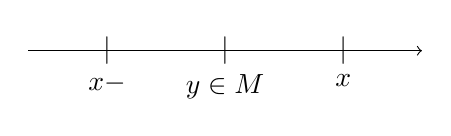
\begin{tikzpicture}[decoration=brace]
\draw[->](0,0)--(5,0);
\foreach \x/\xtext in {1.0/$x-\eps$,2.5/$y \in M$,4.0/$x$}
  \draw(\x,-5pt) node[below] {\xtext} (\x,0pt) node{$|$};
\end{tikzpicture}\\
Nach Lemma 3.13 $\Rightarrow \exists y \in M : x - \eps < y \le x$. Dabei $y^2 \le a$.\\
$x^2-a \le x^2 - y^2 = \underbrace{(x+y)}_{\in (0,2x]} \underbrace{(x-y)}_{\in [0,\eps)} < 2x \eps - x^2 - a$ \wspruch \\
\underline{Annahme 2}: $x^2 < a \Rightarrow \frac{1}{x^2} > 1 \Rightarrow \frac{a}{x^2} -1 > 0$\\
Sei $r := $ min $\left\{1, \frac{1}{3} \cdot \left(\frac{a}{x^2} - 1\right)\right\} > 0 \Rightarrow (1+r)^2 = 1+(2+r) \cdot r < 1 + 3r \le \frac{1}{x^2}$\\
$\Rightarrow (x(1+r))^2 \le a \Rightarrow x(1+r) \in M$, aber $x(1+r) > x$ (\wspruch zu $x=$ sup $M$!)
} \qed

\newpage

\section{Rechenregel für Wurzeln gleichen Exponents}\label{3.17}
Seien $x,y \in \R$ und $x,y > 0$ und $k \in \N \Rightarrow \sqrt[k]{x} \cdot \sqrt[k]{y} = \sqrt[k]{xy}$

\subsection*{Beweis}
$\left(\sqrt[k]{x} \cdot \sqrt[k]{y}\right)^k = \left(\sqrt[k]{x}\right)^k \cdot \left(\sqrt[k]{y}\right)^k = x \cdot y$ (Behauptung)\nl
Wir wissen: $\sqrt{2} \in \R \setminus \Q$. Also $\Q \subset \R \wedge \Q \neq \R$ ($\R$ ist bedeutend größer!).\\
Die Zahlen aus $\R \setminus \Q$ heißen irrational.

\subsection*{Bemerkung}
Im Körper $\Q$ ist das Vollständigkeitsaxiom \underline{nicht} erfüllt, das heißt es gibt beschränkte Mengen $M \subsetneq \Q$, so dass $M$ kein Supremum in $\Q$ hat.\\
Denn sonst würde 3.16 auch in $\Q$ gelten $\Rightarrow x^2=2$ hätte eine Lösung in $\Q$ \wspruch

\subsection*{Beispiel}
$\{y \in \Q : y > 0 \wedge y^2 \le 2 \}$ hat kein Supremum in $\Q$.

\newpage

\chapter{Funktionen}\label{P4}
\section{Definition: Funktionen, Abbildungen}\label{4.1}
Seien $X, Y$ Mengen. Eine \underline{Abbildung} \emph{(=Funktion)} $f$ von $X$ nach $Y$ ist eine Vorschrift, die jedem $x \in X$ genau ein $y=f(x) \in Y$ zuordnet.

\subsection*{Schreibweise}
$f: X \to Y, x \mapsto f(x)$\\
$X$: Definitionsbereich von $f$\\
$Y$: Ziel-, Wertebereich von $f$\\
$f(x)$: Bild von $x$ unter $f$ (Wert von $f$ in $x$)

\phantomsection
\addcontentsline{toc}{section}{Graph von f}
\section*{\texorpdfstring{Graph von $f$}{Graph von f}}
$\Gamma_f=\{(x,f(x)): x \in X\} \subseteq X \times Y$ \nl
\includegraphics[scale=0.5]{img/2013-10-28/1}
\includegraphics[scale=0.5]{img/2013-10-28/2}\\
Beachte: Bei jedem $x \in X$ (im rechten Bild) startet genau ein Pfeil!

\subsection*{Bezeichnung}
Der Begriff ``Funktion'' ist insbesondere gängig, falls $X$ und $Y$ Mengen von Zahlen sind.